\newpage 
\section{Cost--Latency Tradeoff}
\label{app:cost-latency}
% We study the cost--latency tradeoff of Speculative Action, where at each time step the Speculator could launch multiple speculative branches in parallel, each proposing a candidate next tool-call. 
\subsection{Breadth-focused speculation details}
Algorithm 1 launches $k$ parallel speculative branches at any step $t\in\{1,\dots,T-1\}$, which is then immediately followed  with an API call. We assume each branch independently produces the correct next call with probability $p$. Let
\[
p(k) := \Pr(\text{at least one branch is correct}) 
= 1 - (1-p)^k.
\]

We assume the latency of a speculative call is $\mathrm{Exp}(\alpha)$, and the latency of a real API call is $\mathrm{Exp}(\beta)$ with $\beta < \alpha$. Let $c$ denote the cost per unit time for both speculation and real API work. Let
\[
\E[T_{\mathrm{spec}}],\quad \E[M_{\mathrm{spec}}]
\]
denote the expected latency and cost under Algorithm~1 (1 step breadth speculation), and similarly let $(T_{\mathrm{seq}},M_{\mathrm{seq}})$ denote the sequential process with no speculation.

\vspace{3pt}
\begin{theorem}[Cost--Latency Tradeoff for Breadth Speculation]
\label{thm:cost-latency-tradeoff}
Under the setup above,
\begin{align*}
    \frac{E[T_{\mathrm{seq}} - T_{\mathrm{spec}}]}{E[T_{\mathrm{seq}}]}
    \;=\;&\frac{1}{T}\frac{\alpha}{\alpha+\beta}\left[\frac{(T-1)p(k)}{1+p(k)}+\frac{p(k)^2}{(1+p(k))^2} - \frac{p(k)^2}{(1+p(k))^2}(-p(k))^{T-1}\right]\\
    &\xrightarrow{\;\;T\to\infty\;\;}
    \frac{p(k)}{1+p(k)}\cdot\frac{\alpha}{\alpha+\beta}
\end{align*}

For cost, letting $\tilde{k}$ denote the number of \emph{distinct} actions produced across the $k$ speculative branches,
\begin{align*}
    \frac{\E[M_{\mathrm{spec}} - M_{\mathrm{seq}}]}{\E[M_{\mathrm{seq}}]}
    &=\tilde{k}
    -\frac{1}{T}\left(\tilde{k}+\frac{\alpha}{\alpha+\beta}\right)
    \left[
        \frac{(T-1)p(k)}{1+p(k)}
        +\frac{p(k)^2}{(1+p(k))^2}
        -\frac{p(k)^2}{(1+p(k))^2}(-p(k))^{T-1}
    \right]
    \\
    &\xrightarrow{T\to\infty}
    \tilde{k}
    -
    \left(\tilde{k}+\frac{\alpha}{\alpha+\beta}\right)
    \frac{p(k)}{1+p(k)}.
\end{align*}
Note that $\tilde{k}$ is possibly different from $k$ because the $k$ independent speculations might have duplications, in which case we kill the duplicated speculation processes.
\end{theorem}

\begin{proof}
 The proof of the time savings ratio is given in Appendix~\ref{app:proof}. For cost, we have
    \[M_{seq} \propto \frac{T}{\beta}\]
    \[M_{spec} \propto \frac{T}{\beta}(\tilde{k}+1) - S_{T-1}\left(\tilde{k}\frac{1}{\beta} +\frac{\alpha}{\beta(\alpha+\beta)}\right)\]
    where the speculative expression is due to each hit by time step $T-1$ will result in (i) the cached next step not having a speculative window, hence does not launch any speculations (ii) over counting hit action's generation time with execution time.

    Plug in expressions we obtained from Appendix~\ref{app:proof}, we get the expression desired.
\end{proof}

% \paragraph{Interpretation.}
% In the above analysis, we can see that the cost ratio $\left(\tilde{k}+\frac{\alpha}{\alpha+\beta}\right)
%     \frac{p(k)}{1+p(k)}$ and latency ratio $\frac{p(k)}{1+p(k)}\cdot\frac{\alpha}{\alpha+\beta}$, both governed by $p(k)$ with respect to a change in $k$, poses a fundamental tradeoff between the latency gains and the cost induced with extra calls.

% \begin{remark}
%     Note that the above speculation framework could be interpreted as a breadth-focused search, where each speculation is immediately followed by a real API call, hence with depth 1. In the next section, we analyze the other extreme where we do depth-focused search.
% \end{remark}


\subsection{Additional Empirical Results}
\label{app:additional-empiricals}
% \subsubsection{Chess}
% \begin{table}[h!]
% \centering
% \small
% \setlength{\tabcolsep}{4pt}
% \begin{tabular}{c|c|cccc}
% \hline
% \textbf{Number of Speculations} & \textbf{Metric} & 20 steps & 30 steps & 40 steps & 50 steps \\
% \hline
% 1 & Time Saved Percentage (\%) & 6.00 & 8.30 & 5.89 & 4.35 \\
%  Speculation & Extra Tokens used (\%) & 91.82 & 90.73 & 93.45 & 91.00 \\
% \hline
% 2 & Time Saved Percentage (\%) & 16.51 & 17.99 & 14.38 & 11.44 \\
%   Speculations& Extra Tokens used (\%) & 148.98 & 147.96 & 158.69 & 161.26 \\
% \hline
% 3 & Time Saved Percentage (\%) & 28.11 & 30.96 & 23.52 & 19.32 \\
% Speculations  &Extra Tokens used (\%) & 171.64 & 166.06 & 191.26 & 192.13 \\
% \hline
% Confidence-based & Time Saved Percentage (\%) & \textbf{21.97} & \textbf{24.53} & \textbf{18.95} & \textbf{16.18} \\
%  selective launch & Extra Tokens used (\%) & \textbf{90.97} & \textbf{90.11} & \textbf{87.14} & \textbf{84.89} \\
% \hline
% \end{tabular}
% \end{table}

% \begin{figure}[h]
%     \centering
%     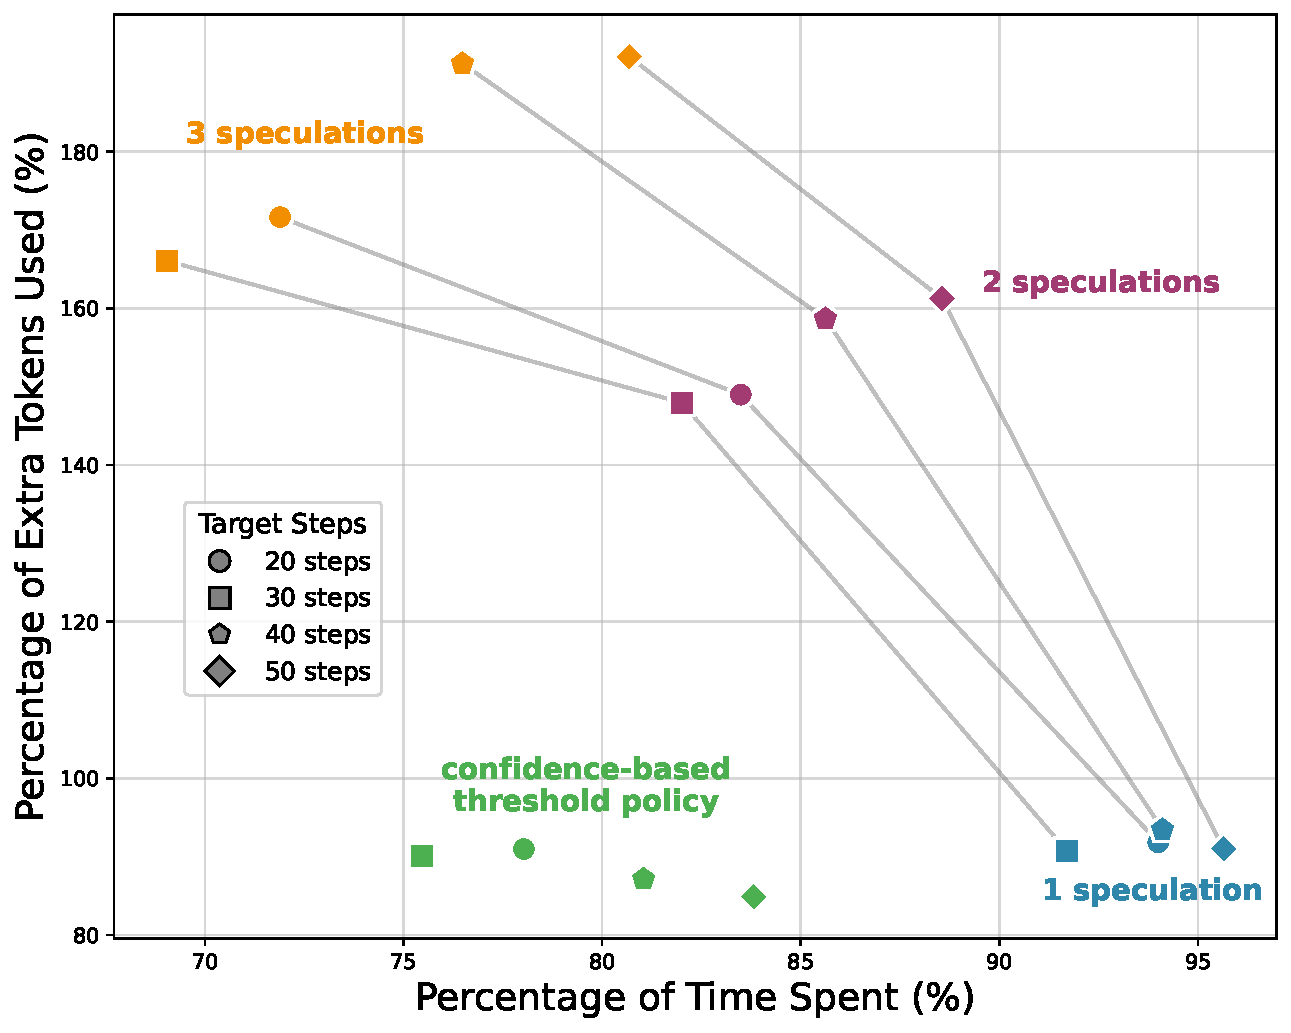
\includegraphics[width=0.7\linewidth]{figures/chess/plot_with_confidence.pdf}
%     \caption{Cost-latency tradeoff across different speculation numbers. With confidence prediction heuristic described above, we are able to achieve lowest cost with comparable time save as 3 predictions, outperforming 2 and 1 predictions.}
%     \label{fig:tradeoff}
% \end{figure}

% \paragraph{Trade-off between Time Saved and Token Cost.} In addition to time savings, we also measure the additional token cost of parallel speculation. We track this using the metric \textbf{extra token percentage}: $(M_{speculative} -M_{sequantial})/{M_{sequential}}$. Figure~\ref{fig:tradeoff} shows the trade-off between time saved and token cost for each number of predictions. We observe that the extra token percentage increases as the number of predictions increases, while the time saved percentage also increases, creating a clear trade-off. Additionally, we observe through the 1,2,3 prediction pattern that there is a non-linear increase cost increase ratio, as consistent with Theorem~\ref{thm:cost-latency-tradeoff}: as $k$ increases, the coefficient $1/1+p(k)$ decreases, thus creating a non-linear dependence.


\subsubsection{E-commerce}

\paragraph{Trade-off between Prediction Accuracy and Cost.}
The time cost in Figure~\ref{fig:time_acc} consists of latency (Time to First Token) and output response time. The dashed vertical line represents the average user typing time, estimated at 40 words per minute. At this threshold, the multi-agent setting achieves approximately 34\% prediction accuracy, meaning that in over one-third of cases the agent can return an immediate response without waiting for API execution. This demonstrates that speculation can transform user experience from perceptibly laggy to effectively real-time in tool-heavy environments.

\begin{figure}[H]
  \centering
  \resizebox{0.8\textwidth}{!}{%
      \begin{subfigure}[t]{0.48\textwidth}
        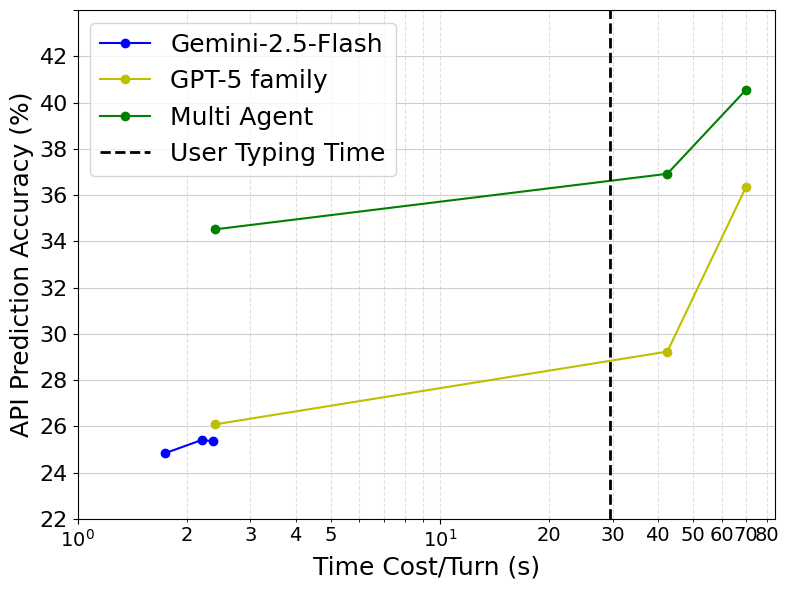
\includegraphics[width=\linewidth]{figures/ecommerce/time_accuracy.png}
        \caption{}
        \label{fig:time_acc}
      \end{subfigure}
      \hspace{0.05\textwidth} 
      \begin{subfigure}[t]{0.48\textwidth}
        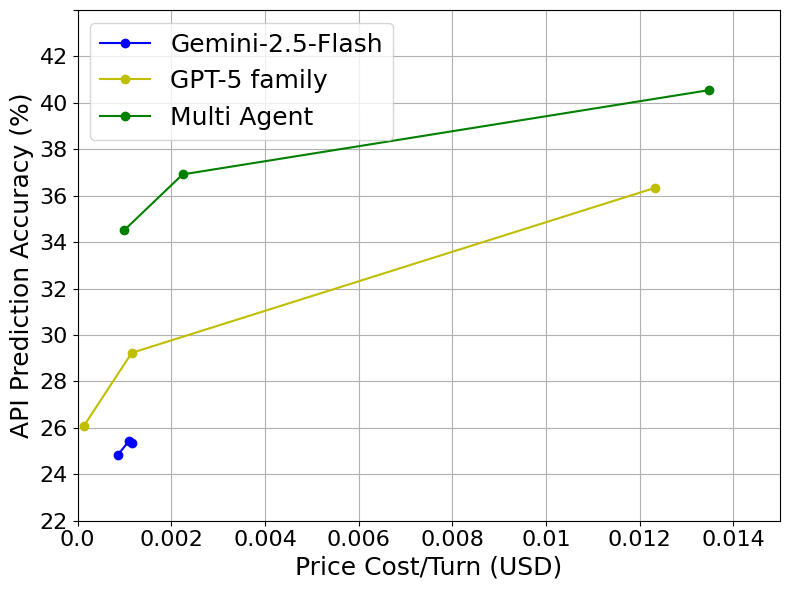
\includegraphics[width=\linewidth]{figures/ecommerce/price_accuracy.png}
        \caption{}
        \label{fig:price_acc}
      \end{subfigure}
  }
  \caption{\textbf{Prediction Accuracy against Speculator's Cost across different models.} (a) Accuracy–Speculator time cost trade-off across models. The dashed line shows average user typing time. (d) Accuracy–Speculator price trade-off across models, reflecting the monetary cost of speculative execution.}
  \vspace{-1em}
\end{figure}


\subsubsection{OS hyperparameter tuning}

\begin{figure*}[h]
  \centering
  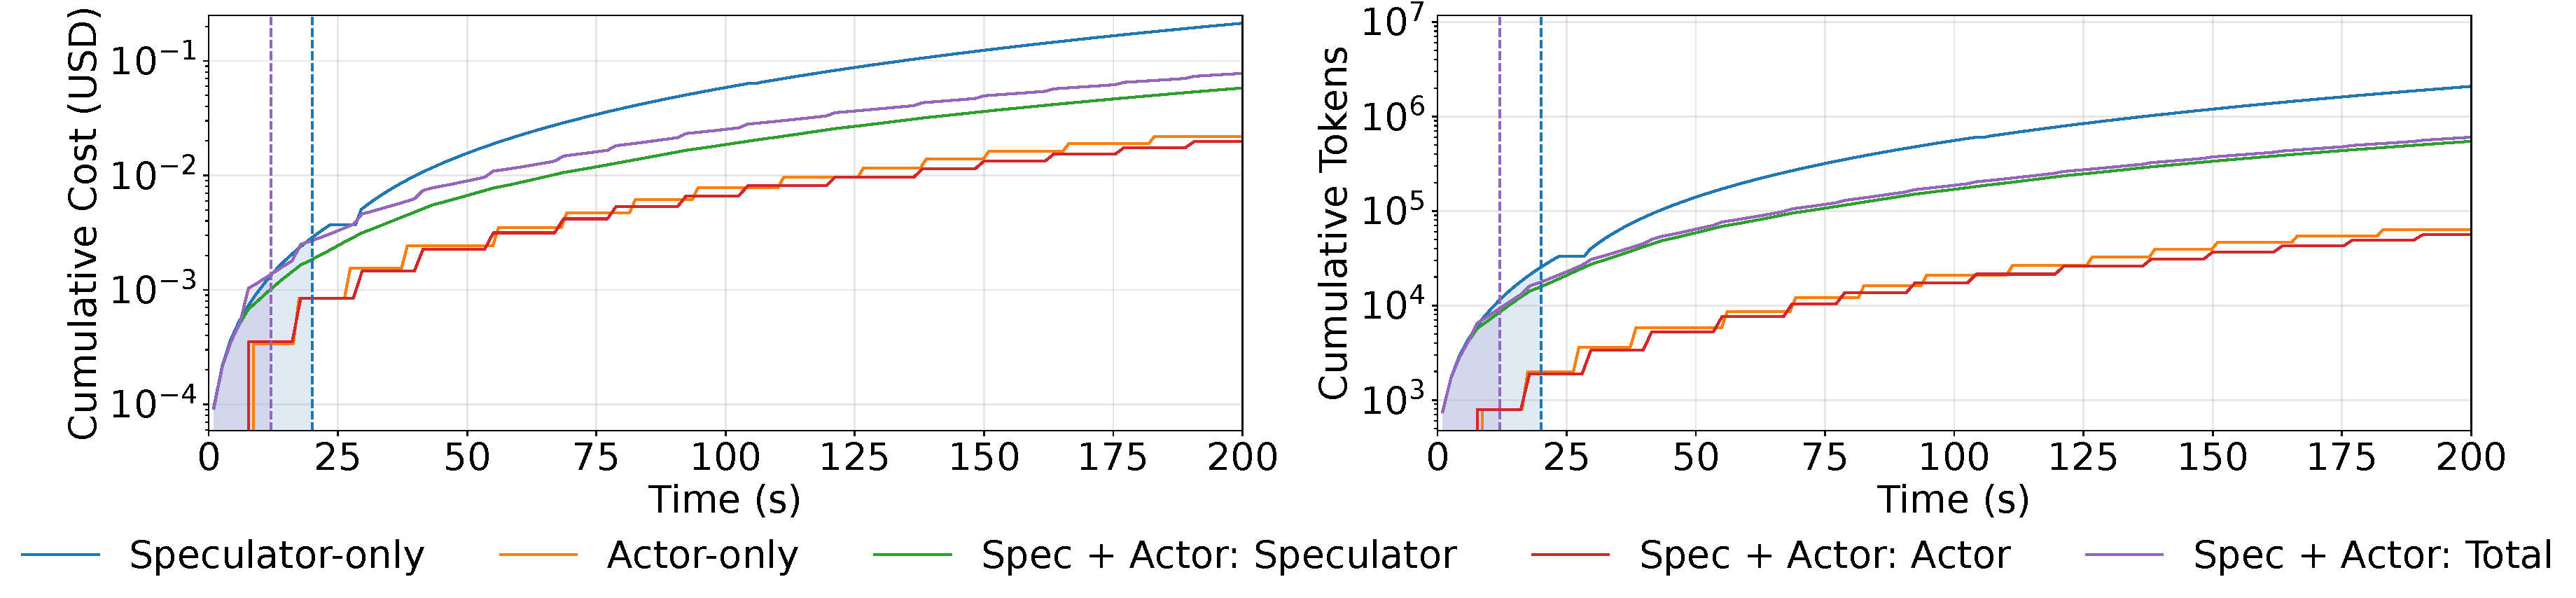
\includegraphics[width=\linewidth]{figures/os_tuning/cost.pdf}
  \caption{\textbf{Cumulative token usage and cost over time.}
  The left and right plots show the cumulative cost (USD) and total tokens used, respectively, for all three configurations.
  The vertical lines mark the observed convergence point for each system. The Actor-only model converges at 200s}
  \label{fig:costs}
\end{figure*}


\begin{table*}[ht]
\centering
\caption{Cumulative tokens and cost (in cents) at selected time marks. While Speculation incurs higher instantaneous costs, its rapid convergence (bolded) prevents long-term resource waste compared to the slower Actor-only baseline.}
\label{tab:costs}
\begin{tabular}{lrrrrrr}
\toprule
& \multicolumn{2}{c}{Actor-only} & \multicolumn{2}{c}{Speculator-only} & \multicolumn{2}{c}{Actor+Speculator (Total)} \\
\cmidrule(lr){2-3}\cmidrule(lr){4-5}\cmidrule(lr){6-7}
\textbf{Elapsed Time} & \textbf{Tokens} & \textbf{Cost (cents)} & \textbf{Tokens} & \textbf{Cost (cents)} & \textbf{Tokens} & \textbf{Cost (cents)} \\
\midrule
Base Prompt  & 744   & 0.02 & 690 & 0.01 & 1434 & 0.03 \\
\textbf{\textcolor{mypurple}{13s}} 
  & 1,216 & 0.05 & 14,973 & 0.18 
  & \textbf{\textcolor{mypurple}{12,135}} 
  & \textbf{\textcolor{mypurple}{0.17}} \\
\textbf{\textcolor{myblue}{20s}} 
  & 2,211 & 0.09 
  & \textbf{\textcolor{myblue}{27,654}} 
  & \textbf{\textcolor{myblue}{0.34}} 
  & 20,504 & 0.31 \\
30s & 3,631   & 0.15 & 45,768 & 0.57 & 32,459 & 0.48 \\
60s & 8,581   & 0.35 & 205,794  & 2.24 & 84,568 & 1.18 \\
120s  & 26,398 & 0.96 & 778,253  & 8.12 & 261,855  & 3.53 \\
\textbf{\textcolor{myred}{200s}} 
  & \textbf{\textcolor{myred}{63,376}} 
  & \textbf{\textcolor{myred}{2.18}} 
  & 2,099,894 & 21.5 & 607,877 & 7.83 \\
\bottomrule
\end{tabular}
\caption{}
\label{tab:os}
\end{table*}

\noindent \textbf{Impact of Context Strategy on Cost.} 
While the Speculator operates at high frequency, the cost overhead is mitigated by the history compression mechanism described in \S\ref{app:history_os}. 
In the combined system, the expensive Actor model reads only a compressed summary of the Speculator's many steps, rather than the raw verbose logs. 
This keeps the prompt size for the Actor relatively stable compared to a linear growth of uncompressed history. 
As a result, the cost difference between the Actor-only and Speculator+Actor systems is driven primarily by the number of Speculator calls, rather than an explosion in context size per call.

As illustrated in Figure~\ref{fig:costs} and detailed in Table~\ref{tab:costs}, the high frequency of the Speculator leads to rapid growth in token consumption and cost. 
In practice, however, this growth is bounded by the system's fast convergence. 
The combined Actor-Speculator system converges in approximately 13 seconds, while the Speculator-only system converges in 20 seconds. The Actor-only system converges after 200 seconds. 
Once an optimal state is reached, the tuning process concludes, rendering the potential for long-term exponential cost negligible in this context. Several optimization strategies, like truncating the context to a fixed window or disabling exploration after convergence, could further mitigate token growth but are left for future work.

\subsection{Confidence-Aware Speculation}

We formalize the branch selection problem introduced in
Section~\ref{subsec:dynamic-speculation}.

\paragraph{Model.}
Fix a horizon $T$ and an integer $k \ge 1$.
At each epoch $t$, the system is in mode $z_t \in \{0,1\}$:
\begin{itemize}
    \item $z_t = 0$: a speculation window is available,
    \item $z_t = 1$: a cached correct action must be executed (no speculation).
\end{itemize}

Let $a$ and $b$ denote the actor and speculator latencies, respectively, and define the latency gain
\[
\ell := a - b > 0,
\]
which is collected only at epochs with $z_t = 1$.

\paragraph{Accuracy process.}
At epochs with $z_t = 0$, an accuracy vector
$\mathbf P_t = (P_t^1,\dots,P_t^k) \in [0,1]^k$
is realized and observed.
Assume $\mathbf P_t \sim F_t$ independently across $t$,
where the distribution $F_t$ may vary over time.

Given a realization $\mathbf p$, let
$p^{(1)} \ge \dots \ge p^{(k)}$
denote the sorted coordinates.

\paragraph{Action and hit probability.}
At $z_t = 0$, the agent chooses $m_t \in \{0,\dots,k\}$,
launching the top $m_t$ branches at cost $c m_t$.
The probability of obtaining a cached action is
\[
q(m;\mathbf p)
=
1 - \prod_{j=1}^{m} (1 - p^{(j)}),
\qquad
q(0;\mathbf p) = 0.
\]

\paragraph{Mode transition.}
If $z_t = 1$, then $z_{t+1} = 0$ deterministically.
If $z_t = 0$ and action $m$ is chosen,
\[
z_{t+1} =
\begin{cases}
1, & \text{w.p. } q(m;\mathbf P_t), \\
0, & \text{w.p. } 1 - q(m;\mathbf P_t).
\end{cases}
\]

\paragraph{Reward.}
The per-epoch reward is
\[
R_t =
\begin{cases}
\ell, & z_t = 1, \\
- c m_t, & z_t = 0.
\end{cases}
\]
The objective is to maximize
$\mathbb E\!\left[\sum_{t=1}^T R_t\right]$.


We then present the proof to the first part (general non-stationary) of Theorem~\ref{thm:dynamic}.

\begin{proof}
Let $V_t^{(z)}$ denote the optimal expected total reward from epochs
$t,\dots,T$ given mode $z_t=z$,
with terminal conditions
$V_{T+1}^{(0)} = V_{T+1}^{(1)} = 0$.

By standard dynamic programming arguments,
the Bellman equations are
\begin{align}
V_t^{(1)} &= \ell + V_{t+1}^{(0)}, \label{eq:bellman1} \\
V_t^{(0)} &=
\mathbb E_{\mathbf P \sim F_t}
\Big[
\max_{m \in \{0,\dots,k\}}
\big\{
- c m
+ q(m;\mathbf P)\,V_{t+1}^{(1)}
+ (1-q(m;\mathbf P))\,V_{t+1}^{(0)}
\big\}
\Big].
\label{eq:bellman0}
\end{align}

Define the continuation gap
\[
\Delta_t := V_{t+1}^{(1)} - V_{t+1}^{(0)}.
\]

Substituting \eqref{eq:bellman1} into \eqref{eq:bellman0} yields
\[
V_t^{(0)}
=
V_{t+1}^{(0)}
+
\mathbb E_{\mathbf P \sim F_t}
\Big[
\max_m
\{ q(m;\mathbf P)\,\Delta_t - c m \}
\Big].
\]

Hence, conditional on observing $\mathbf p$ at epoch $t$,
the optimal decision maximizes
\[
q(m;\mathbf p)\,\Delta_t - c m,
\]
establishing the stated policy.

Finally, using
\[
\Delta_t
=
V_{t+1}^{(1)} - V_{t+1}^{(0)}
=
\ell + V_{t+2}^{(0)} - V_{t+1}^{(0)},
\]
and substituting the expression for $V_{t+1}^{(0)}$
gives the scalar recursion
\[
\Delta_t
=
\ell
-
\mathbb E_{\mathbf P \sim F_{t+1}}
\Big[
\max_m \{ q(m;\mathbf P)\,\Delta_{t+1} - c m \}
\Big],
\]
with terminal condition $\Delta_T = 0$ (or equivalently, $\Delta_{T-1} = \ell$).
\end{proof}

% \begin{remark}[Mean-only approximation]
% Suppose only the mean accuracy vectors
% $\mu_t := \mathbb E_{F_t}[\mathbf P_t]$
% are available.
% Let $\mu_t^{(1)} \ge \dots \ge \mu_t^{(k)}$ denote the sorted coordinates,
% and define
% \[
% \bar q_t(m)
% =
% 1 - \prod_{j=1}^{m} (1 - \mu_t^{(j)}).
% \]

% Replacing the expectation in the scalar recursion by this
% certainty-equivalent hit probability yields
% \[
% \tilde\Delta_T = \ell,
% \qquad
% \tilde\Delta_t
% =
% \ell
% -
% \max_{m \in \{0,\dots,k\}}
% \{ \bar q_{t+1}(m)\,\tilde\Delta_{t+1} - c m \}.
% \]

% The resulting implementable policy is
% \[
% \tilde m_t(\mathbf p)
% \in
% \arg\max_{m}
% \{ q(m;\mathbf p)\,\tilde\Delta_t - c m \}.
% \]

% This approximation is exact if $F_t$ is degenerate at its mean,
% and otherwise serves as a computationally light surrogate.
% \end{remark}
% \begin{lemma}[Marginal-threshold form of the stationary policy]
% Fix a constant $\Delta^\star>0$ and per-branch cost $c>0$.
% Given a realization $\mathbf p=(p^1,\dots,p^k)$, let
% $p^{(1)}\ge \cdots \ge p^{(k)}$ be the sorted probabilities and define
% \[
% q(m;\mathbf p) := 1-\prod_{j=1}^{m}(1-p^{(j)}), \qquad q(0;\mathbf p)=0,
% \]
% and the incremental hit probability
% \[
% \delta q(m;\mathbf p) := q(m+1;\mathbf p)-q(m;\mathbf p)
% = \left(\prod_{j=1}^{m}(1-p^{(j)})\right)p^{(m+1)}.
% \]
% Then any maximizer
% \[
% m^\star(\mathbf p)\in\arg\max_{m\in\{0,\dots,k\}}\{q(m;\mathbf p)\Delta^\star-cm\}
% \]
% satisfies the marginal cutoff condition
% \[
% \Delta^\star \cdot \delta q(m;\mathbf p)\ \ge\ c \quad \text{for all } m<m^\star(\mathbf p),
% \qquad
% \Delta^\star \cdot \delta q(m;\mathbf p)\ \le\ c \quad \text{for all } m\ge m^\star(\mathbf p).
% \]
% Equivalently, $m^\star(\mathbf p)$ can be obtained by the greedy rule:
% starting from $m=0$, repeatedly add the next-best branch $(m+1)$ while
% $\Delta^\star \cdot \delta q(m;\mathbf p)\ge c$, and stop otherwise.
% \end{lemma}

% \naimeng{The other modeling: suppose this is infinite horizon but optimal stopping: each step there is q probability to exit.}
We then formally describe the stationary average reward corollary. 
\begin{corollary}[Stationary infinite-horizon average-reward policy]
Assume the nonstationary model becomes stationary:
\begin{itemize}
    \item $\mathbf P_t \sim F$ i.i.d.\ across $t$,
    \item the hit probability $q(m;\mathbf p)$ and cost $c$ are time-invariant,
    \item the objective is to maximize long-run average reward.
\end{itemize}

Let $\bar q(m) := \mathbb E_{\mathbf P \sim F}[q(m;\mathbf P)]$ denote
the expected hit probability when launching $m$ branches.

Then the optimal average reward $g^\star$ satisfies
\[
g^\star
=
\max_{m \in \{0,\dots,k\}}
\frac{\bar q(m)\,\ell - c m}{1 + \bar q(m)}.
\]

Define
\[
\Delta^\star := \ell - g^\star.
\]

Then an optimal stationary policy at a speculation window is
\[
m^\star(\mathbf p)
\in
\arg\max_{m \in \{0,\dots,k\}}
\{ q(m;\mathbf p)\,\Delta^\star - c m \}.
\]

In particular, the optimal policy mapping (the scalar $\Delta^\star$) is time homogeneous.
\end{corollary}

\begin{proof}
Fix $\Delta^\star>0$. Conditional on observing $\mathbf p$ at a speculation window, the stationary one-step objective is
\[
f(m;\mathbf p) := q(m;\mathbf p)\,\Delta^\star - c m,
\qquad m\in\{0,1,\dots,k\}.
\]
The first display in the corollary is exactly the definition of $m^\star(\mathbf p)$ as any maximizer of $f(m;\mathbf p)$.

To show the greedy marginal-threshold form, note that for sorted confidences
$p^{(1)}\ge\cdots\ge p^{(k)}$,
\[
q(m;\mathbf p)=1-\prod_{j=1}^{m}(1-p^{(j)}),
\]
so the discrete marginal gain from adding the $(m+1)$-th branch is
\[
f(m+1;\mathbf p)-f(m;\mathbf p)
=\Delta^\star\bigl(q(m+1;\mathbf p)-q(m;\mathbf p)\bigr)-c
=\Delta^\star\,\delta q(m;\mathbf p)-c,
\]
where
\[
\delta q(m;\mathbf p)
:=q(m+1;\mathbf p)-q(m;\mathbf p)
=\Big(\prod_{j=1}^{m}(1-p^{(j)})\Big)p^{(m+1)}.
\]
Moreover, $\delta q(m;\mathbf p)$ is nonincreasing in $m$ (diminishing returns), since
$p^{(m+1)}$ is nonincreasing and the prefactor $\prod_{j=1}^{m}(1-p^{(j)})$ is nonincreasing in $m$.
Hence the increments $f(m+1;\mathbf p)-f(m;\mathbf p)$ are nonincreasing in $m$ as well.

Therefore there exists an index $m^\star(\mathbf p)$ such that
$f(m+1;\mathbf p)-f(m;\mathbf p)\ge 0$ for all $m<m^\star(\mathbf p)$ and
$f(m+1;\mathbf p)-f(m;\mathbf p)\le 0$ for all $m\ge m^\star(\mathbf p)$.
Equivalently,
\[
\Delta^\star \cdot \delta q(m;\mathbf p)\ge c \;\;\text{for } m<m^\star(\mathbf p),
\qquad
\Delta^\star \cdot \delta q(m;\mathbf p)\le c \;\;\text{for } m\ge m^\star(\mathbf p),
\]
which is precisely the greedy stopping rule stated in the corollary.
\end{proof}

% \subsubsection{Experimental result}
% % We implement the above heuristic with the chess environment and plot the cost-latency tradeoff
% We implement a threshold policy discussed above in the chess environment. We use the same GPT5 model as the predictor. As shown in figure~\ref{fig:tradeoff}, our policy achieves lowest cost measured by extra tokens used, while achieving latency reduction exceeding both 1 and 2 prediction branchings, falling just short (less than $5\%$) of the latency reduction achieved by launching 3 speculations per step. 



% \subsection{Heuristic Policy for Dynamic Speculation Decisions}

% We now consider a more realistic setting in which, at each step, we observe a per-speculation confidence estimate. Suppose that launching a real API costs $a$ time units, a speculative call costs $b<a$, and each step the system produces $k$ speculative candidates with correctness probabilities $\{p_i^1,\dots,p_i^k\}$.

% Let $r$ and $c$ be the weights placed on latency and monetary cost, respectively, so that we maximize
% \[
% \max_{\pi} \; r\cdot\mathrm{latency} + c\cdot\mathrm{cost}.
% \]

% For a single speculation with correctness probability $p_i$, the decision is whether to \emph{accept} (continue unrolling this speculative branch) or \emph{reject} (discard it and continue sequentially). Let $V(i)$ be the optimal value-to-go at token index $i$.

% If we \textbf{accept} the speculation, the expected one-step reward is
% \begin{align*}
% A(i)
% &=
% p_i\bigl[ r b + c(b+a) + r a + c a + V(i+2)\bigr]
% +
% (1-p_i)\bigl[r a + 2c a + V(i+1)\bigr]
% \\
% &=
% p_i\bigl[ r b + c(b+a) + r a + c a + V(i+2)\bigr]
% + (1-p_i)\bigl[r a + 2c a + V(i+1)\bigr].
% \end{align*}

% If instead we \textbf{reject}, the expected reward is simply
% \[
% R(i) = r a + c a + V(i+1).
% \]

% We propose a simple heuristic: treat all future timesteps as if their speculation correctness probability is the baseline value $p$. Under this approximation the dynamic program becomes stationary, and for long horizons the value function becomes approximately linear, enabling a closed-form threshold policy.

% \subsection{Long-Horizon Approximation and Closed-Form Threshold Policy}



\subsection{Depth focused search}
In the most general setting, a policy may choose both (1) how many parallel speculative branches to launch, and (2) how “deep” to unroll each speculative branch before initiating a real API call. Analyzing the optimal policy in this full space is highly non-trivial due to the branching structure of the execution tree.

To build intuition, we analyze two extrema regimes:
(1) a \emph{breadth-focused} regime, where at each step we launch $k$ parallel speculations and immediately follow each with an API call, and  
(2) a \emph{depth-focused} regime, where execution follows a single branch as far as speculation and real API calls allow. These two settings correspond to simplified extremes of the decision space, providing interpretable analytic characterizations of the cost--latency tradeoff.

We analyzed the first in the previous section, and now analyze the opposite extreme: a depth-focused strategy. Under this policy, whenever either a speculative or real API call returns, the system launches \emph{one} new real call and \emph{one} speculation on top of that branch. If the real API result is inconsistent with the corresponding speculative guess, all descendants of that speculation are discarded. Let $p$ be the per-step correctness probability of a speculative guess.

Assume for simplicity that the real API call latency is deterministically $a$ and a speculative call latency is $b<a$.

\begin{theorem}[Cost--Latency Tradeoff for Depth Speculation]
Let $p$ be the probability that a speculation is correct at each step. Then under the depth-focused policy described above,
\[
    \frac{\E[T_{\mathrm{seq}} - T_{\mathrm{spec}}]}{\E[T_{\mathrm{seq}}]}
    = \frac{T-1}{T} \, p \Bigl(1 - \frac{b}{a}\Bigr),
\]
and the expected cost satisfies
\[
    \frac{\E[M_{\mathrm{spec}} - M_{\mathrm{seq}}]}{\E[M_{\mathrm{seq}}]}
    =
    \frac{T-1}{T}
    \frac{
        (1-p)\left[
            a\lfloor\tfrac{a}{b}\rfloor 
            - b\frac{(1+\lfloor\tfrac{a}{b}\rfloor)\lfloor\tfrac{a}{b}\rfloor}{2}
        \right]
        + p b\lfloor\frac{a}{b}\rfloor
    }{a}\approx\frac{T-1}{T}\left((1-p)\left(\frac{a}{2b}-\frac{1}{2}\right)+p\right)
\]
\label{thm:depth}
\end{theorem}

\begin{proof}
    We directly calculate the expected time cost of speculation execution as follows
    \[T_{spec} = a+ \sum_{s=0}^{T-1}\binom{T-1}{s}p^s(1-p)^{T-1-s}[sb+(T-1-s)a]\]
    Let 
\[
S \sim \mathrm{Binomial}(T-1, p),
\]
so that
\[
\mathbb{P}(S=s) = \binom{T-1}{s} p^s (1-p)^{T-1-s}, 
\quad s = 0, \dots, T-1.
\]

Then
\begin{align*}
&\sum_{s=0}^{T-1} \binom{T-1}{s} p^s (1-p)^{T-1-s}
\bigl[sb + (T-1-s)a\bigr] \\
&= \mathbb{E}\!\left[Sb + (T-1-S)a\right] \\
&= b\,\mathbb{E}[S] + a\,\mathbb{E}[T-1-S].
\end{align*}

Since
\[
\mathbb{E}[S] = (T-1)p,
\]
we obtain
\begin{align*}
b(T-1)p + a\bigl(T -1- (T-1)p\bigr)
&= a(T-1) + (T-1)p(b-a).
\end{align*}

Therefore,
\[T_{spec} = a+ 
\sum_{s=0}^{T-1} \binom{T-1}{s} p^s (1-p)^{T-1-s}
\bigl[sb + (T-s)a\bigr]
= aT + (T-1)p(b-a).
\]
Directly plug in $T_{seq} = aT$, we get the expression desired.

For cost, we know that with $(1-p)$ probability, speculation is inconsistent with true action, and the amount of tokens spent is from the branches that were spawn off before the correct action returns, that is
\begin{align*}
    \text{Token of this step} &= a+(a-b)+(a-2b)+\dots + \left(a-\lfloor\frac{a}{b}\rfloor b\right)\\
    &=a\cdot\left(\lfloor\frac{a}{b}\rfloor+1\right) - \frac{\left(1+\lfloor\frac{a}{b}\rfloor\right)\cdot\lfloor\frac{a}{b}\rfloor}{2}\cdot b
\end{align*}
With probability $p$, speculation matches with true action, in which case
\[\text{Token of this step} = a+ \lfloor\frac{a}{b}\rfloor b\]
Therefore
\begin{align*}
    M_{spec} &= a+ (T-1)\left[p\left(a+ \lfloor\frac{a}{b}\rfloor b\right)+(1-p)\left(a\cdot\left(\lfloor\frac{a}{b}\rfloor+1\right) - \frac{\left(1+\lfloor\frac{a}{b}\rfloor\right)\cdot\lfloor\frac{a}{b}\rfloor}{2}\cdot b\right)\right]
\end{align*}
\end{proof}

\paragraph{Interpretation.}
Note that compared to breadth speculation, Depth speculation produces speedups unbounded in $p$ coefficient (the coefficient in front for breadth is $\frac{1}{2}$ whereas for depth speculation this coefficient is 1). In terms of cost, depth speculation cost has highest order term $(1-p)(\frac{a}{2b}-\frac{1}{2})$. This is governed by how many speculations one can spawn off before the current action is returned. 


